\documentclass{article}

\usepackage{graphicx}
\usepackage{float}


\begin{document}


\begin{titlepage}

\begin{center}
\huge{\small BANGABANDHU SHEIKH MUJIBUR RAHMAN SCIENCE AND TECHNOLOGY UNIVERSITY,GOPALGANJ-8100}\\
[1mm]

\textsc{\small  SHEIKH HASINA INSTITUTE of ICT}\\

\end{center}
\begin{figure}[H]
\centering
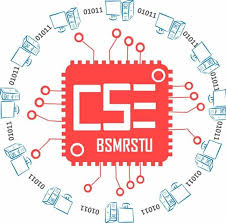
\includegraphics[height=4.00in•]{downloadbsmrstucse.jpg}
\\
\end{figure}
\begin{center}
\textsc{\large CSE-156}\\
A LATEX REPORT\\ ON\\
\textsc{\large DATA MINIG}\\
\end{center}

\begin{flushright}

\textsc{MOMINUL HAQUE\\}
ID NO: 18ICTCSE007\\
A genarel latex user\\
\#123\\
E-mail : nmhaque07@gmail.com\\
27 December 2019


\end{flushright}

\end{titlepage}
\pagenumbering{roman}


\newpage
\section*{Summary}
\addcontentsline{toc}{section}{\numberline{}Summary}
Data Mining is all about explaining the past and predicting the future for analysis.
Data mining helps to extract information from huge sets of data. It is the procedure of mining knowledge from data.
Data mining process includes business understanding, Data Understanding, Data Preparation, Modelling, Evolution, Deployment.
Important Data mining techniques are Classification, clustering, Regression, Association rules, Outer detection, Sequential Patterns, and prediction
R-language and Oracle Data mining are prominent data mining tools.
Data mining technique helps companies to get knowledge-based information.
The main drawback of data mining is that many analytics software is difficult to operate and requires advance training to work on.
Data mining is used in diverse industries such as Communications, Insurance, Education, Manufacturing, Banking, Retail, Service providers, eCommerce, Supermarkets Bioinformatics.
\cleardoublepage
\tableofcontents
\thispagestyle{empty}
\cleardoublepage
\pagenumbering{arabic}
\setcounter{page}{1}
\section{introduction}
\label{sec:intro}
Data mining is looking for hidden, valid, and potentially useful patterns in huge data sets. Data Mining is all about discovering unsuspected/ previously unknown relationships amongst the data.

It is a multi-disciplinary skill that uses machine learning, statistics, AI and database technology.

The insights derived via Data Mining can be used for marketing, fraud detection, and scientific discovery, etc.

Data mining is also called as Knowledge discovery, Knowledge extraction, data/pattern analysis, information harvesting, etc.
\section{Data Mining Softwear Features}
\begin{figure}[H]
\centering
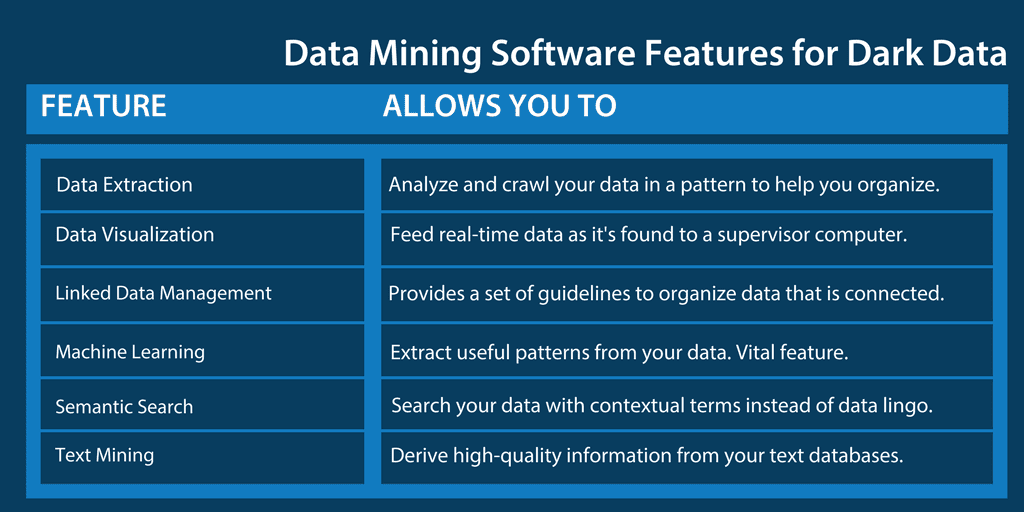
\includegraphics[height=3.35in•]{Data_Mining_Features (1).png}
\caption{0}

\end{figure}


\newpage
\section{Data Mining Implementation Process}
\begin{figure}[H]

\includegraphics[height=.450in•]{data_mining_2.png}
\caption{Let's study the Data Mining implementation process in detail}
\centering\section{Types of Data}

Data mining can be performed on following types of data\\
[2mm]
\subsection{Relational databases}
\subsection{Data warehouses}
\subsection{Advanced DB and information repositories}
\subsection{Object-oriented and object-relational databases}
\subsection{Transactional and Spatial databases}
\subsection{Heterogeneous and legacy databases}
\subsection{Multimedia and streaming database}
\subsection{Text databases}
\subsection{Text mining and Web mining}

\end{figure}


\section{Business understanding:}
\subsection{\small First, you need to understand business and client objectives.\\ You need to define what your client wants (which many times even they do not know themselves)}
\subsection{\small Take stock of the current data mining scenario. Factor in resources,\\ assumption, constraints, and other significant factors into your assessment.}
\subsection{\small business objectives and current scenario, define your data mining goals.}
\paragraph{Data understanding:}
\subparagraph{$first, data is collected from multiple data sources available in the organization\\These data sources may include multiple databases, \\flat filer or data cubes. There are issues like object\\ matching and schema integration which\\ can arise during Data Integration process. It is a quite complex\\ and tricky process as data from various sources unlikely to match easily.\\ For example, table A contains an entity \\named cust_no whereas another table B contains an entity named cust-id.\\
Therefore, it is quite difficult to ensure that both \\of these given objects refer to the same value or\\ not. Here, Metadata should be used\\ to reduce errors in the data integration process.
Next, the step\\ is to search for properties of acquired data. A good way to explore the data is to answer\\ the data mining questions (decided in business phase) using the query, reporting, \\and visualization tools.
Based on the results of query,\\ the data quality should be ascertained. Missing data if any should be\\ acquired.$}

\section{Data preparation:}
\subsection{The data preparation process consumes about 90 of the time of the project.}
\subsection{The data from different sources should be selected, cleaned, transformed, \\formatted, anonymized, and constructed (if required).}
\subsection{Data cleaning is a process to "clean" the data by smoothing noisy data and filling \\in missing values.}
\subsection{For example, for a customer demographics profile, age data is missing. The data\\ is incomplete and should be filled. In some cases,\\ there could be data outliers. For instance, age has a\\ value 300. Data could be inconsistent. \\For instance, name of the customer is different in different tables.}
\subsection{Data transformation operations change the data to make it useful in data mining.\\Following transformation can be applied}
\section{Data transformation:}
\subsection*{Smoothing:\small It helps to remove noise from the data. }
\subsection*{Aggregation:\small Summary or aggregation operations are applied to the data. I.e., the weekly sales data is aggregated to calculate the monthly and yearly total.}
\subsection*{Generalization:\small In this step, Low-level data is replaced by higher-level concepts with the help of concept hierarchies. For example, the city is replaced by the county.}
\subsection*{Normalization:\small Normalization performed when the attribute data are scaled up o scaled down. Example: Data should fall in the range -2.0 to 2.0 post-normalization.}
\subsection*{Attribute construction: \small these attributes are constructed and included the given set of attributes helpful for data mining.\\The result of this process is a final data set that can be used in modeling.}
\newpage

\paragraph{Modelling}
\subparagraph{In this phase, mathematical models are used to determine data patterns.\\Based on the business objectives, suitable modeling techniques should be selected for the prepared dataset.\\Create a scenario to test check the quality and validity of the model.\\Run the model on the prepared dataset.\\Results should be assessed by all stakeholders to make sure that model can meet data mining objectives.}
\paragraph{Evaluation:}
\subparagraph{In this phase, patterns identified are evaluated against the business objectives.\\Results generated by the data mining model should be evaluated against the business objectives.\\Gaining business understanding is an iterative process. In fact, while understanding, new business requirements may be\\raised because of data mining.\\A go or no-go decision is taken to move the model in the deployment phase.}
\newpage
\paragraph{Deployment:}
\subparagraph{In the deployment phase, you ship your data mining discoveries to everyday business operations.\\The knowledge or information discovered during data mining process should be made easy to understand for non-technical stakeholders.\\A detailed deployment plan, for shipping, maintenance, and monitoring of data mining discoveries is created.\\A final project report is created with lessons learned and key experiences during the project. This helps to improve the organization's business policy.}
\section{Programming Code}
\subsection*{simple adding two values}
\#include<stdio.h>\\
main()\\
\{
\\int a=4,b=3\\
print"a+b"\\
\}
\begin{table}
\centering
\caption{Data Mining Applications}
\label{tab:tab 1}
\begin{tabular}{|c|r|}

 \hline Appication &Usage\\ \hline
Communications & Data mining techniques are used in communication sector to predict\\\hline
Insurance & Data mining helps insurance companies to price their products profitable \\\hline
Education & Data mining benefits educators to access student data, predict achievement levels\\\hline
Manufacturing &	With the help of Data Mining Manufacturers can predict wears tear of production.\\\hline
\end{tabular}
\end{table}
\section{Data Mining Techniques}
\begin{figure}[H]
\centering
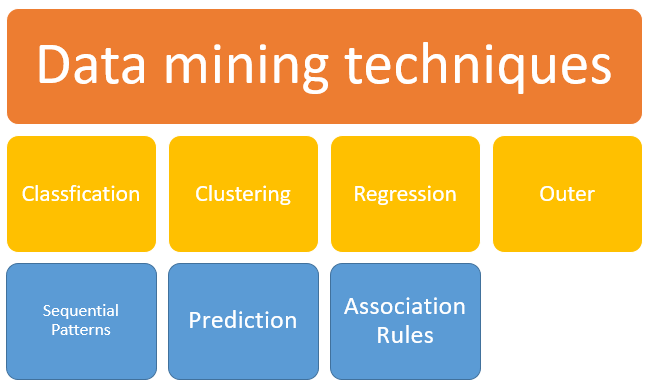
\includegraphics[height=2.35in•]{data_mining_1.png}
\caption{Data Mining Techniques}

\end{figure}
\paragraph*{1.Classification:}
\subparagraph{This analysis is used to retrieve important and relevant information about data, and\\metadata. This data mining method helps to classify data in different classes.}
\paragraph*{2. Clustering:}
\subparagraph{Clustering analysis is a data mining technique to identify data that are like each other.\\This process helps to understand the differences and similarities between the data.}
\paragraph{3. Regression:}
\subparagraph{Regression analysis is the data mining method of identifying and analyzing the relationship between variables. It is used to identify the likelihood of a specific variable, given the presence of other variables.}
\paragraph*{4. Association Rules:}
\subparagraph{This data mining technique helps to find the association between two or more Items. It discovers a hidden pattern in the data set.}
\paragraph*{5. Outer detection:}
\subparagraph{This type of data mining technique refers to observation of data items in the dataset which do not match an expected pattern or expected behavior. This technique can be used in a variety of domains, such as intrusion, detection, fraud or fault detection, etc. Outer detection is also called Outlier\\Analysis or Outlier mining.}
\paragraph*{6. Sequential Patterns:}
\subparagraph{This data mining technique helps to discover or identify similar patterns or trends in transaction data for certain period.}
\paragraph*{7. Prediction:}
\subparagraph{Prediction has used a combination of the other data mining techniques like trends,\\sequential patterns, clustering, classification, etc. It analyzes past events or instances in a right\\sequence for predicting a future event.}
\end{document}
